%%%%%%%%%%%%%%%%%%%%%%%%%%%%%%%%%%%%%%%%%%%%%%%%%%%%%%%%%%%%%%%%     
%%%%%%%%%%%%%%%%%%%%%%%%%%%%%%%%%%%%%%%%%%%%%%%%%%%%%%%%%%%%%%%%
%																															 %
%				USE THIS TEMPLATE, AMETSOC.STY, AND AMETSOC.BST				 %
%			        OR YOUR TEX FILES WILL NOT BE USED				  		 %
%																															 % 
%%%%%%%%%%%%%%%%%%%%%%%%%%%%%%%%%%%%%%%%%%%%%%%%%%%%%%%%%%%%%%%%
%%%%%%%%%%%%%%%%%%%%%%%%%%%%%%%%%%%%%%%%%%%%%%%%%%%%%%%%%%%%%%%%

%%%%%%%%%%%%%%%%%%%%%%%%%%%%%%%%%%%%%%%%%%%%%%%%%%%%%%%%%%%%%%%%%%%%%
% PREAMBLE
%%%%%%%%%%%%%%%%%%%%%%%%%%%%%%%%%%%%%%%%%%%%%%%%%%%%%%%%%%%%%%%%%%%%%
%
% The following two commands will generate a PDF that follows all the requirements for submission
% and peer review.  Uncomment these commands to generate this output (and comment out the two lines below.)
%
% DOUBLE SPACE VERSION FOR SUBMISSION TO THE AMS
\documentclass[12pt]{article}
\usepackage{ametsoc}
\usepackage{epsf,amsfonts,amsmath}
%
% The following two commands will generate a single space, double column paper that closely
% matches an AMS journal page.  Uncomment these commands to generate this output (and comment
% out the two lines above. FOR AUTHOR USE ONLY. PAPERS SUBMITTED IN THIS FORMAT WILL BE RETURNED
% TO THE AUTHOR for submission with the correct formatting.
%
% TWO COLUMN JOURNAL PAGE LAYOUT FOR AUTHOR USE ONLY
%\documentclass[10pt]{article}
%\usepackage{ametsoc2col}
\usepackage{subfigure}
%
%%%%%%%%%%%%%%%%%%%%%%%%%%%%%%%%%%%%%%%%%%%%%%%%%%%%%%%%%%%%%%%%%%%%%
% ABSTRACT
%
% Enter your Abstract here
%%%%%%%%%%%%%%%%%%%%%%%%%%%%%%%%%%%%%%%%%%%%%%%%%%%%%%%%%%%%%%%%%%%%%
\newcommand{\myabstract}{The Boulder repository GSI code is coupled with the WRF tangent linear adjoint model and the GSI-based WRF 4DVAR has been developed. Several experiments are conducted to validate this 4DVAR system and all results confirm the performance of the GSI-based 4DVAR system.}
%
\begin{document}
%
%%%%%%%%%%%%%%%%%%%%%%%%%%%%%%%%%%%%%%%%%%%%%%%%%%%%%%%%%%%%%%%%%%%%%
% TITLE
%
% Enter your TITLE here
%%%%%%%%%%%%%%%%%%%%%%%%%%%%%%%%%%%%%%%%%%%%%%%%%%%%%%%%%%%%%%%%%%%%%
\title{\textbf{\large{Report on the Development of GSI-based WRF 4DVAR \\ ACAPS 2010 SoW Task 3.1.b}}}
%
% Author names, with corresponding author information. 
% [Update and move the \thanks{...} block as appropriate.]
%
\author{\textsc{Xin Zhang}
				%\thanks{\textit{Corresponding author address:} 
				%Dr. Xin Zhang, NCAR/MMM, P.O. Box 3000, 
				 %Boulder, CO 80307. 
				%\newline{E-mail: xinzhang@ucar.edu}}
             \textsc{and Xiang-Yu Huang}\\
\textit{\footnotesize{MMM, National Center for Atmospheric Research, Boulder, CO 80305}}
%\and 
%\centerline{\textsc{Nils Gustafsson}}\\% Add additional authors, different insitution
%\centerline{\textit{\footnotesize{Swedish Meteorological and Hydrological Institute, SE-60176 Norrk�oping, Sweden}}}
}
%
% The following block of code will handle the formatting of the title page depnding on whether
% we are formatting a double column (dc) author draft or a single column paper for submission.
% AUTHORS SHOULD SKIP OVER THIS... There is nothing to do in this section of code.
\ifthenelse{\boolean{dc}}
{
\twocolumn[
\begin{@twocolumnfalse}
\amstitle

% Start Abstract (Enter your Abstract above.  Do not enter any text here)
\begin{center}
\begin{minipage}{13.0cm}
\begin{abstract}
	\myabstract
	\newline
	\begin{center}
		\rule{38mm}{0.2mm}
	\end{center}
\end{abstract}
\end{minipage}
\end{center}
\end{@twocolumnfalse}
]
}
{
\amstitle
\section*{Acknowledgements}
\large{\textit{We would like to thank {\bf{Dr. Ricardo Todling}} for his help to kick off the project and {\bf{Dr. Thomas Auligne, Dr. Junmei Ban, Mrs. Xiaoyan Zhang, Mr. Feng Gao}} for their help and encouragement.}}
\newpage
\begin{abstract}
\myabstract
\end{abstract}
\newpage
}
%%%%%%%%%%%%%%%%%%%%%%%%%%%%%%%%%%%%%%%%%%%%%%%%%%%%%%%%%%%%%%%%%%%%%
% MAIN BODY OF PAPER
%%%%%%%%%%%%%%%%%%%%%%%%%%%%%%%%%%%%%%%%%%%%%%%%%%%%%%%%%%%%%%%%%%%%%
%

\section{Upgrades of WRF tangent linear and adjoint model}

To couple the WRF tangent linear and adjoint model (WRFPLUS) with GSI, the subroutine interfaces for WRF tangent linear and adjoint have been constructed. Some other subroutines, such as  save/read basic states, perturbations and adjoint forcing are also coded. Furthermore, the WRFPLUS has been upgraded to the latest WRF repository and the adjoint check can achieve 15-16 digital identical.  Now, we are working on the parallelization of WRFPLUS.


\section{Coupling GSI with WRFPLUS}

A module named wrf\_pertmod.F90, has been coded to sever as the coupler or hub between GSI and WRFPLUS. It is the only new add-on file in source codes. It includes the interfaces to call WRF, WRF\_TL and WRF\_AD separately. It also includes the subroutines conducting the transfer of state variables between GSI space and WRF space and their adjoint.

At this moment, the GSI-based WRF 4DVAR can run with 1-processor parallel run due to the undergoing WRFPLUS parallelization. We have tested the system on IBM with XLF compiler and Linux with PGI compiler.

\section{Single Observation test}

4DVAR approach has the capability to implicitly evolve the static background error statistics. Single observation is the best way to demonstrate the  property of 4DVAR. The analysis time is 2000-01-25-00 and the 4DVAR time window is 6 hours. A single 500mb temperature at (32.5,-72, marked as a red star) is assimilated at the end of the time window on 2000-01-25-06. Figure \ref{single} shows the hourly increments between the 6-hour control run (from first guess) and analysis run (from 4DVAR analysis).

\begin{figure}
\includegraphics[scale=0.8]{single1.pdf}
\caption{Hourly increment evolution from 0h to 6h}
\label{single}
\end{figure}

The maximum of analysis increment at 0h is on the upstream and it evolved with time follow the wind stream. Eventually, at the end of time window, the maximum arrives the observation location and the pattern of the increment has the flow dependent property.

\section{3-day real case}

A 3-day CONUS domain, see Figure \ref{domain}, are setup to run experiments to verify the performance of the GSI-based WRF 4DVAR system. The domain size is 47x32x28L, horizontal resolution is 135km; The Initial conditions and boundary conditions at every 6h are prepared from 2007-09-10-00 to 2007-09-13-00 and the initial conditions are the 12h forecast from NCEP FNL analysis; the NCEP GDAS prepbufr data will be used in assimilation.

We ran 3 experiments to compare the performance of the data assimilation. The first experiment is the CONTROL run without data assimilation, 48h forecast are made four times per day. The second experiment (3DVAR)is the 48h forecast from 3DVAR analysis four times per day. The third experiment (4DVAR) is the 48h forecast from 4DVAR analysis four times per day. Then, all the 48h forecasts are verified again the NCAR archived LITTLE\_R format observation.

Figure \ref{0h} to Figure \ref{48h} show the profile RMSE from 0h to 48h forecast. At 0h, the 3DVAR gets the smallest profile RMSE overall as 3DVAR uses more observations in 0h that 4DVAR; At 6h,  4DVAR is the best, it is reasonable because 4DVAR uses the observations at 6h; In the subsequent forecast, 4DVAR experiment wins the verification and confirm our expectation. In the future, we will conduct higher resolution and longer period runs to further confirm the benefit of the 4DVAR.

\begin{figure}
\begin{center}
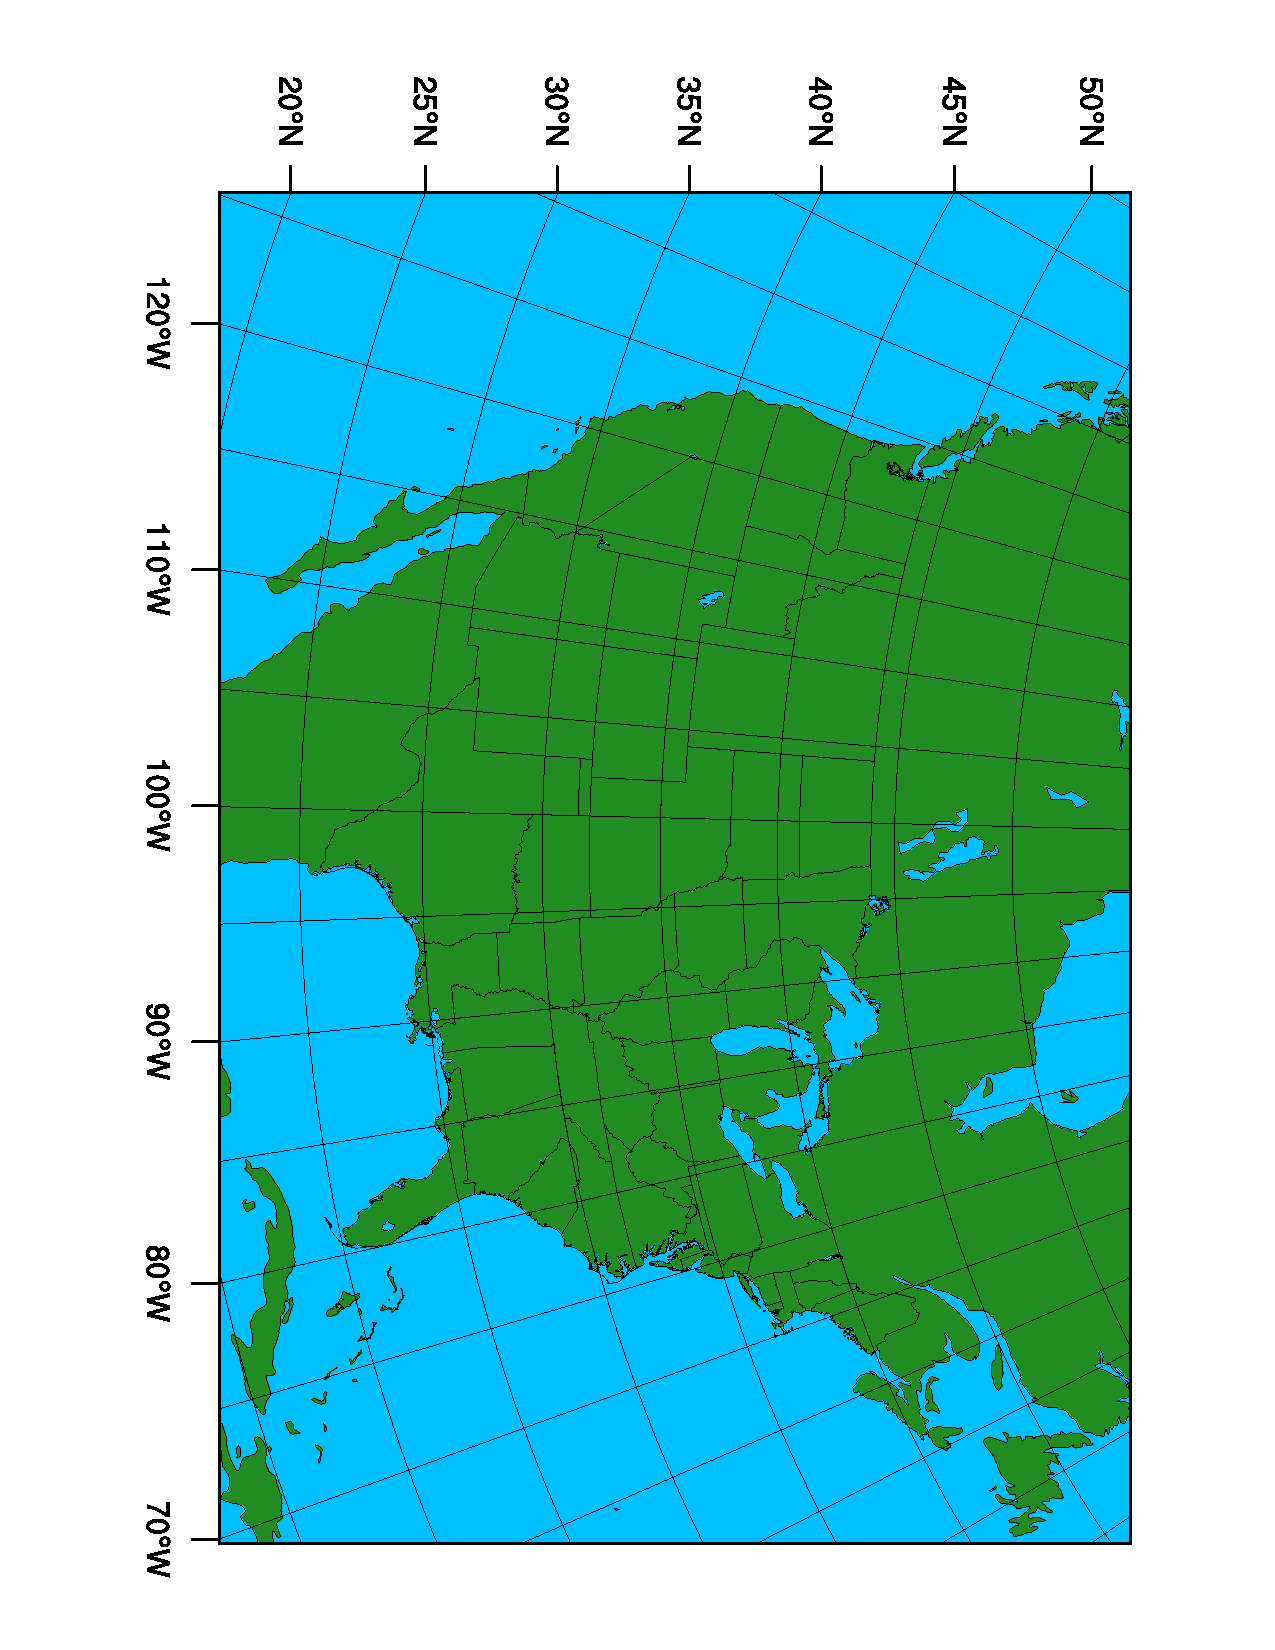
\includegraphics[scale=0.5,angle=90]{domain.pdf}
\caption{domain configuration}
\label{domain}
\end{center}
\end{figure}

\begin{figure}
\begin{center}
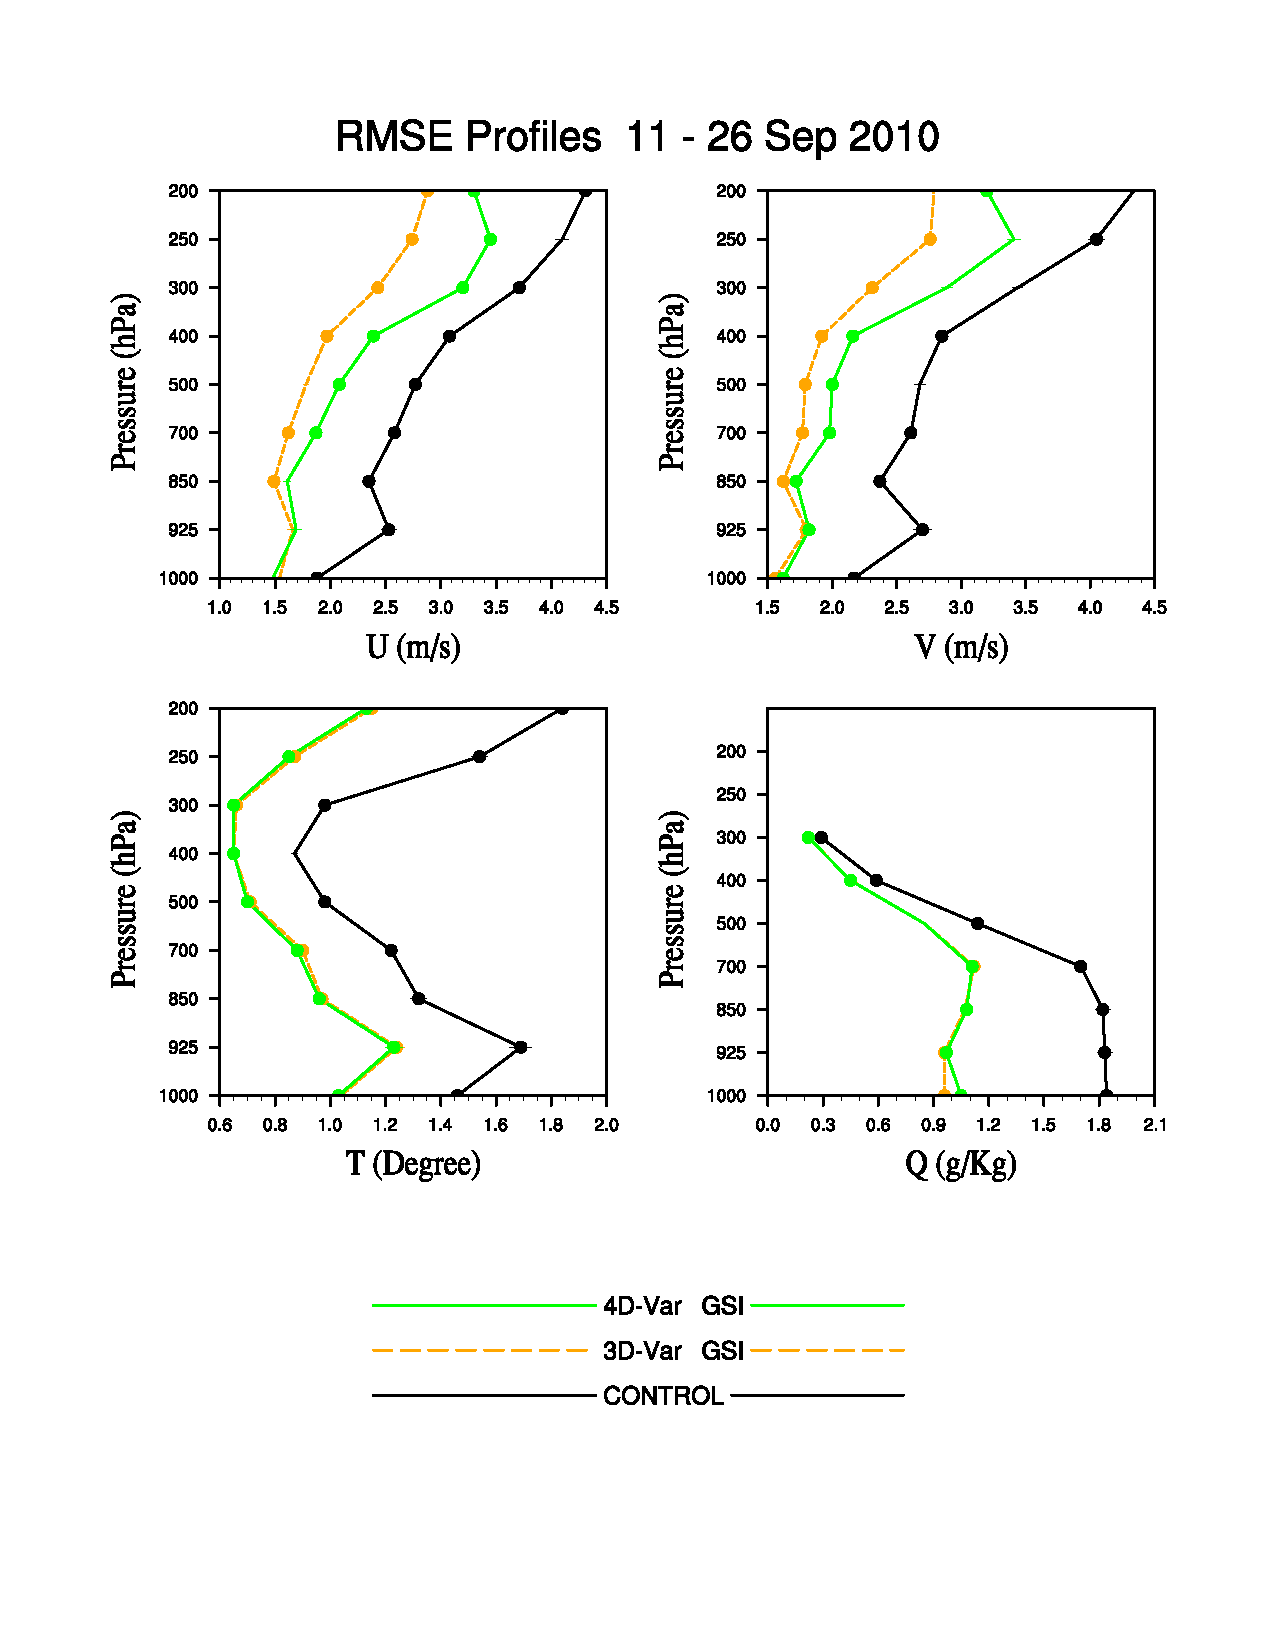
\includegraphics[scale=0.8, trim=0 50 0 80, clip]{Profile_RMSE_0.pdf}
\caption{Profile RMSE at 0h}
\label{0h}
\end{center}
\end{figure}

\begin{figure}
\begin{center}
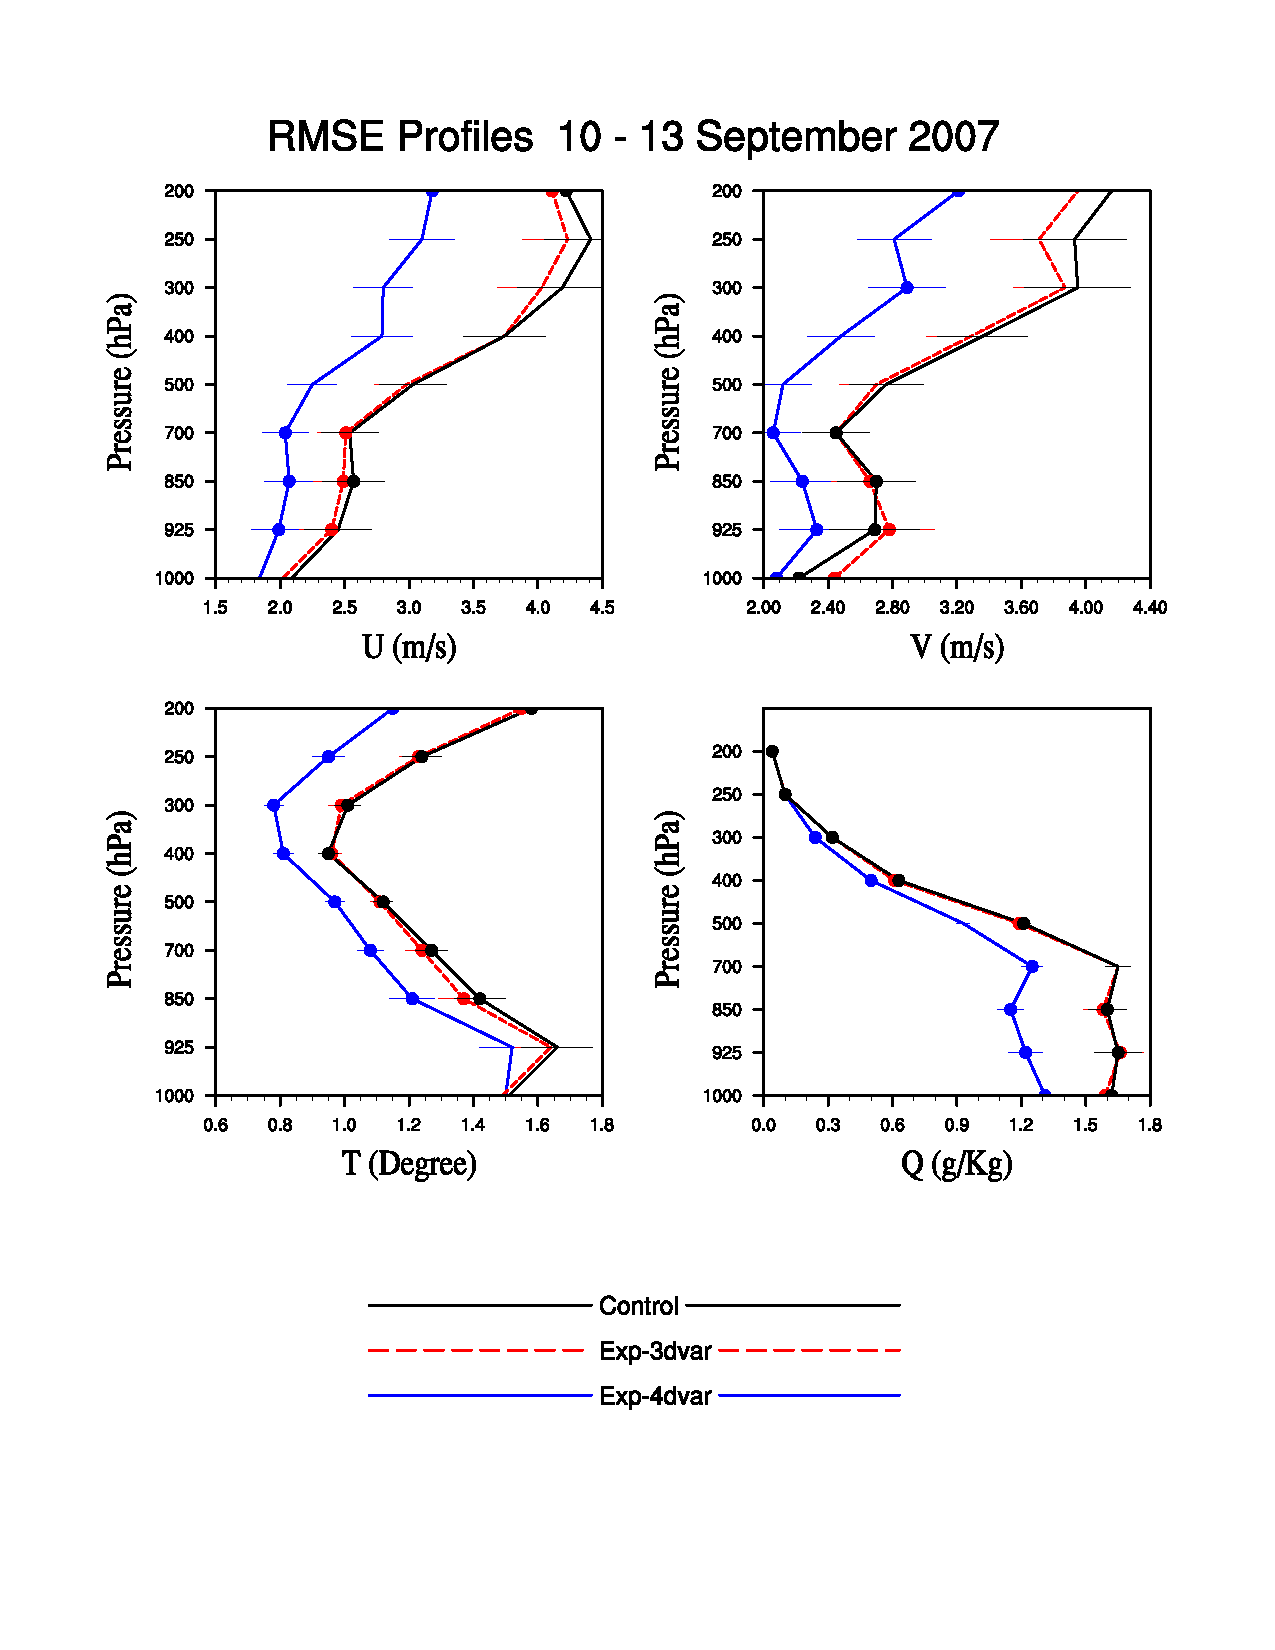
\includegraphics[scale=0.8, trim=0 50 0 80, clip]{Profile_RMSE_6.pdf}
\caption{Profile RMSE at 6h}
\label{6h}
\end{center}
\end{figure}

\begin{figure}
\begin{center}
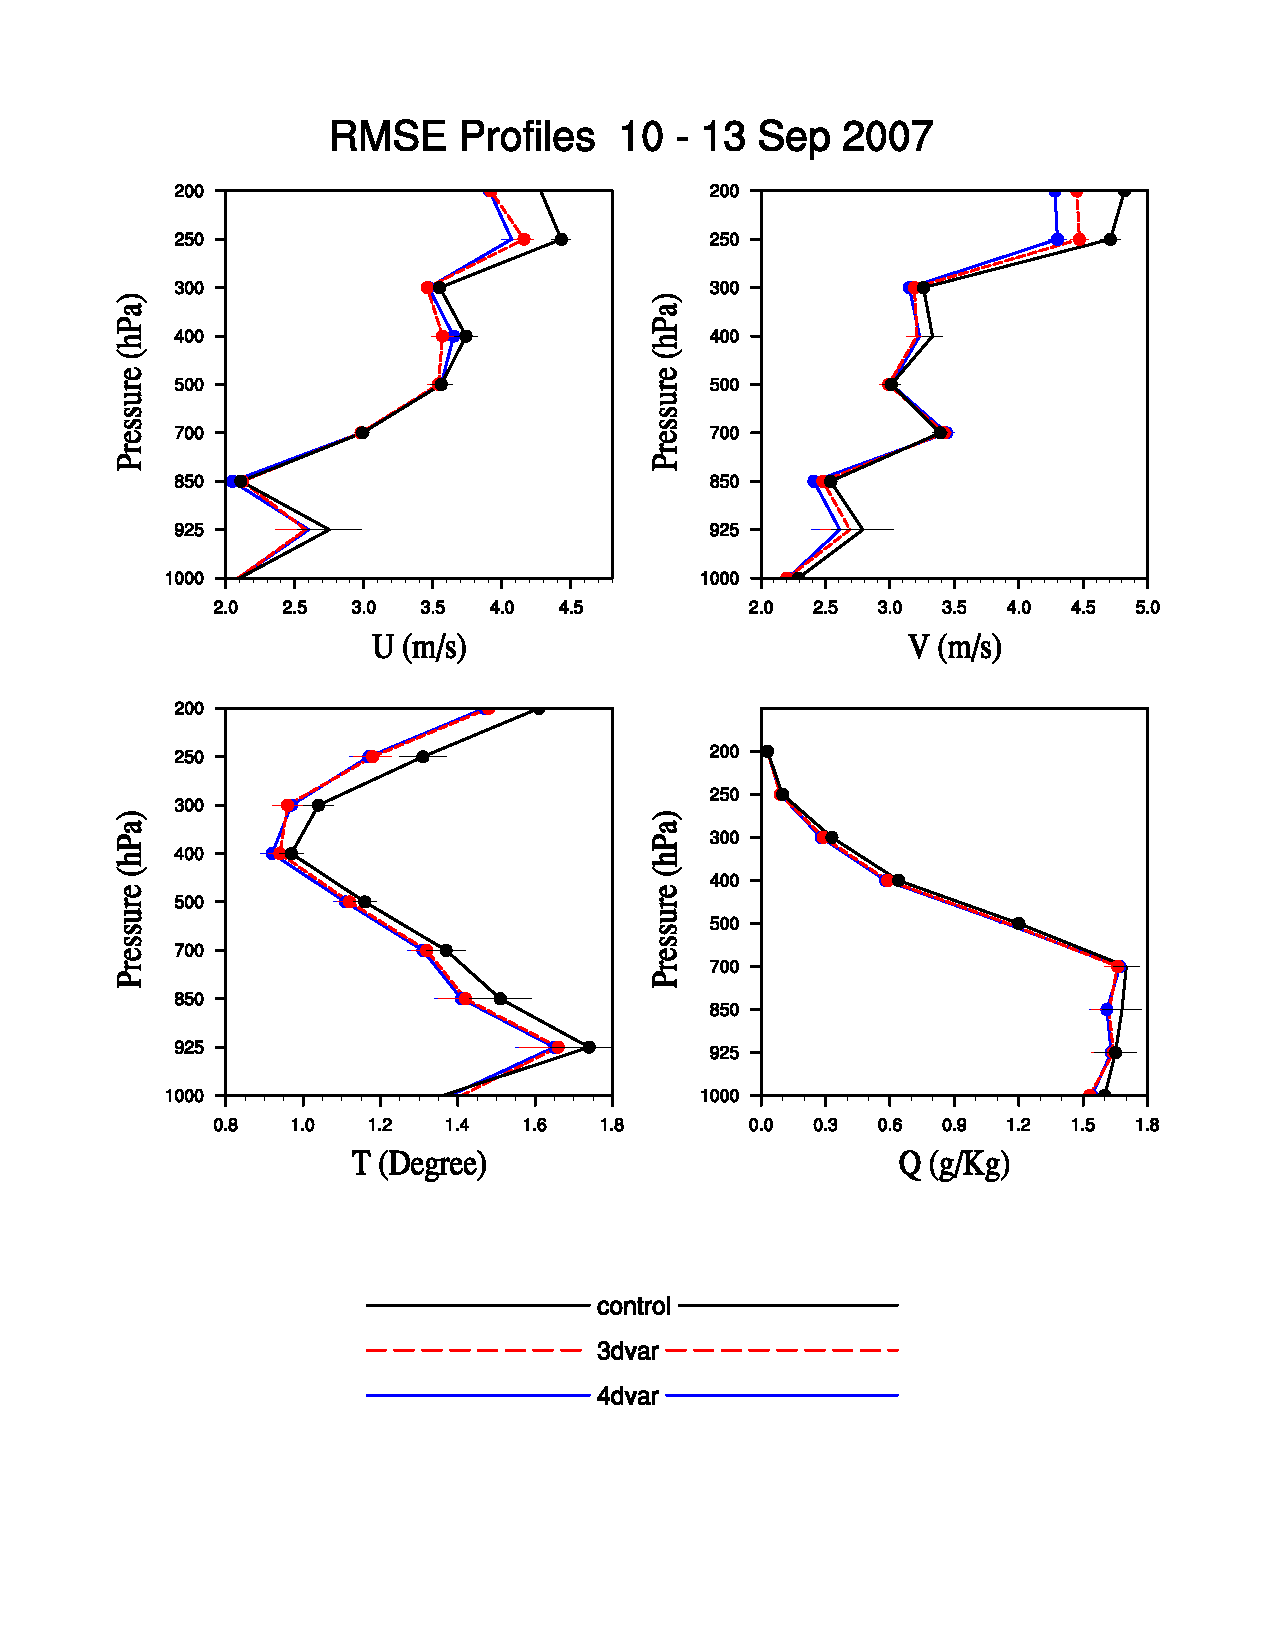
\includegraphics[scale=0.8, trim=0 50 0 80, clip]{Profile_RMSE_12.pdf}
\caption{Profile RMSE at 12h}
\label{12h}
\end{center}
\end{figure}

\begin{figure}
\begin{center}
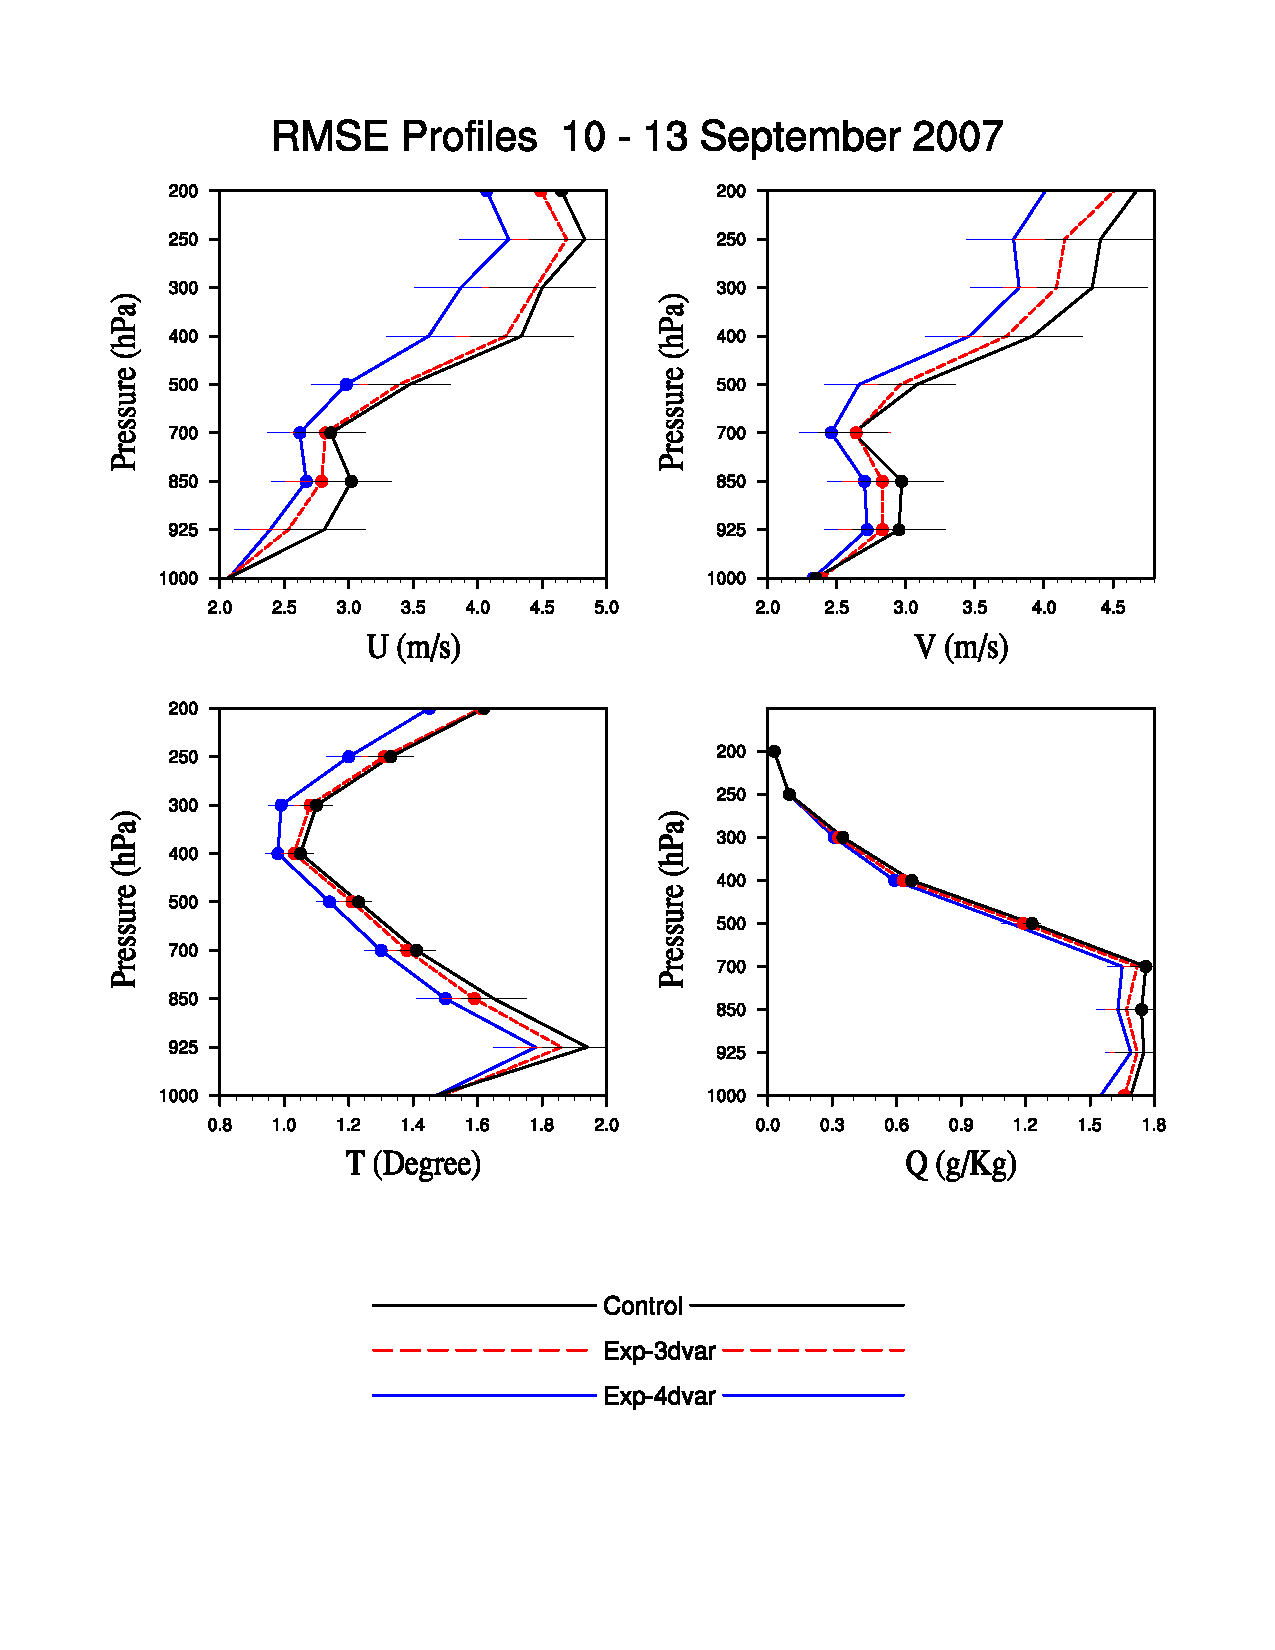
\includegraphics[scale=0.8, trim=0 50 0 80, clip]{Profile_RMSE_18.pdf}
\caption{Profile RMSE at 18h}
\label{18h}
\end{center}
\end{figure}

\begin{figure}
\begin{center}
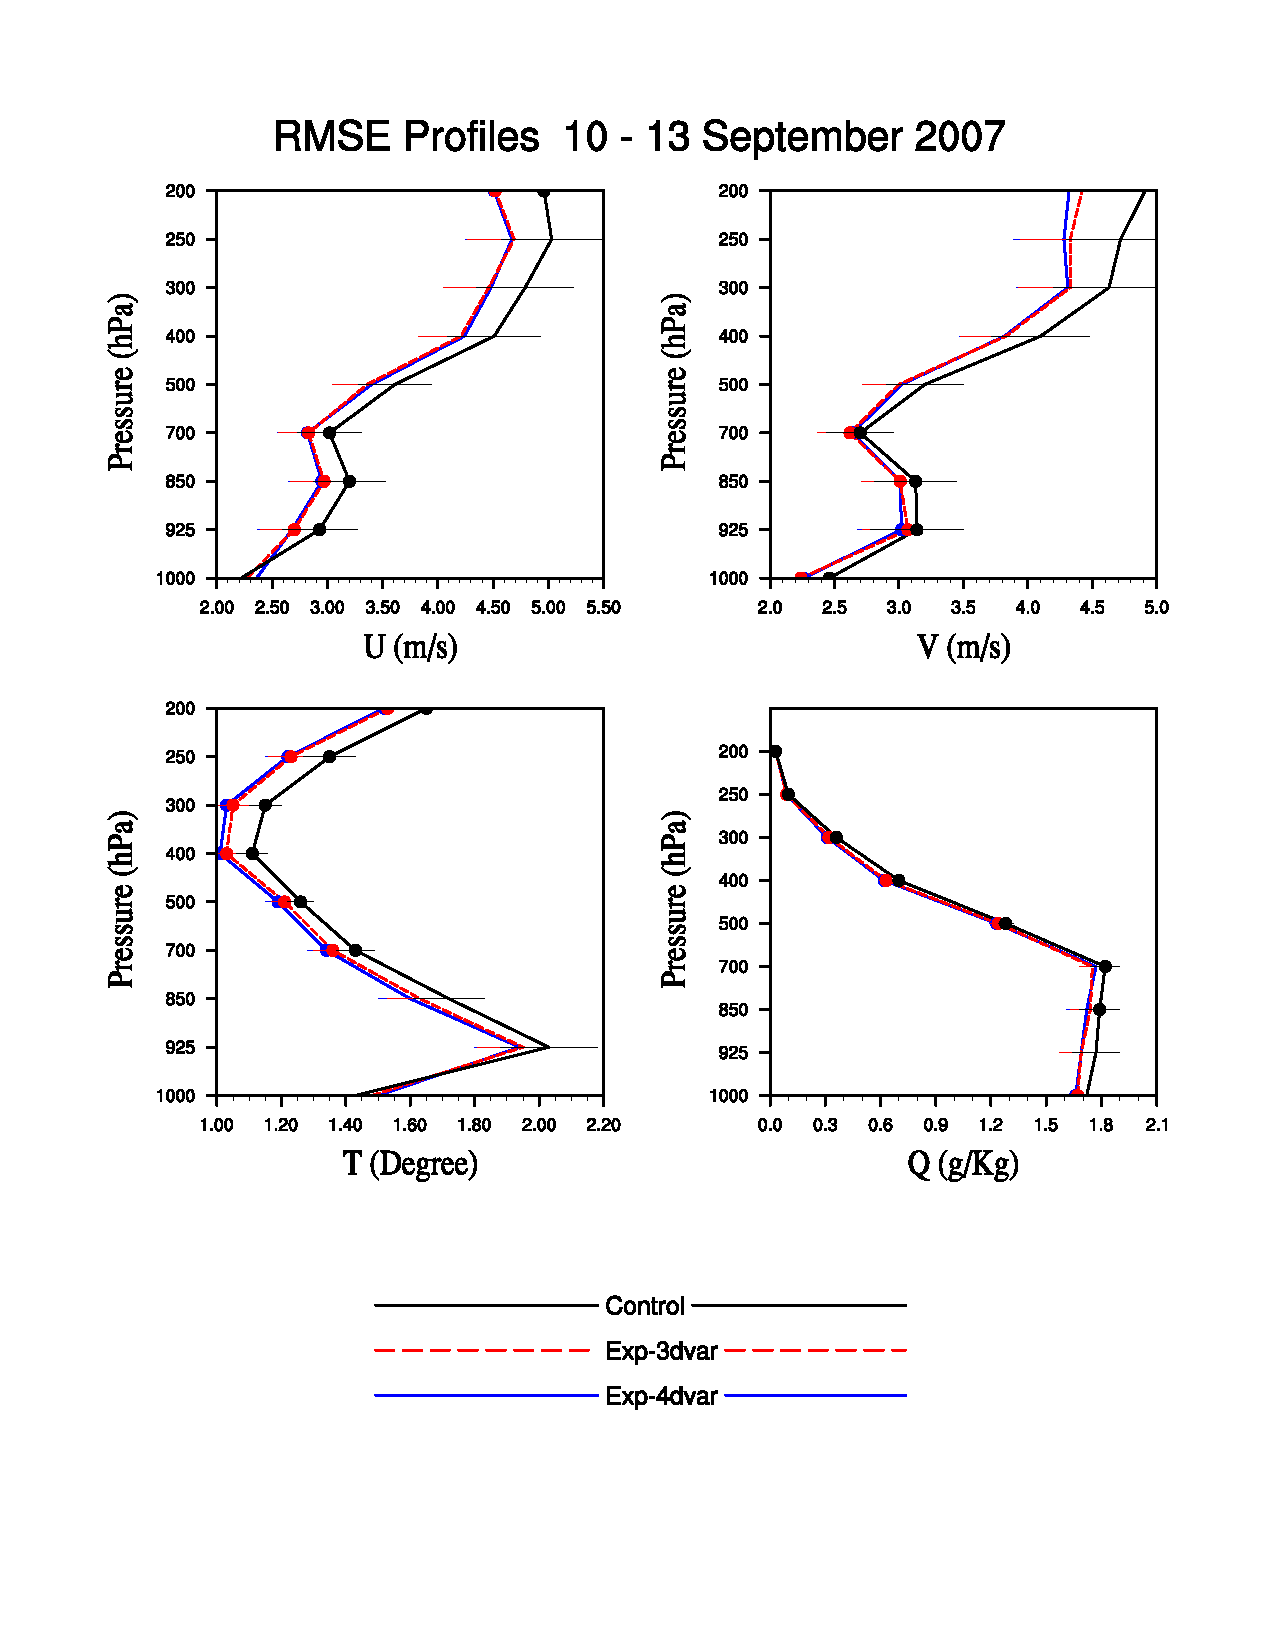
\includegraphics[scale=0.8, trim=0 50 0 80, clip]{Profile_RMSE_24.pdf}
\caption{Profile RMSE at 24h}
\label{24h}
\end{center}
\end{figure}

\begin{figure}
\begin{center}
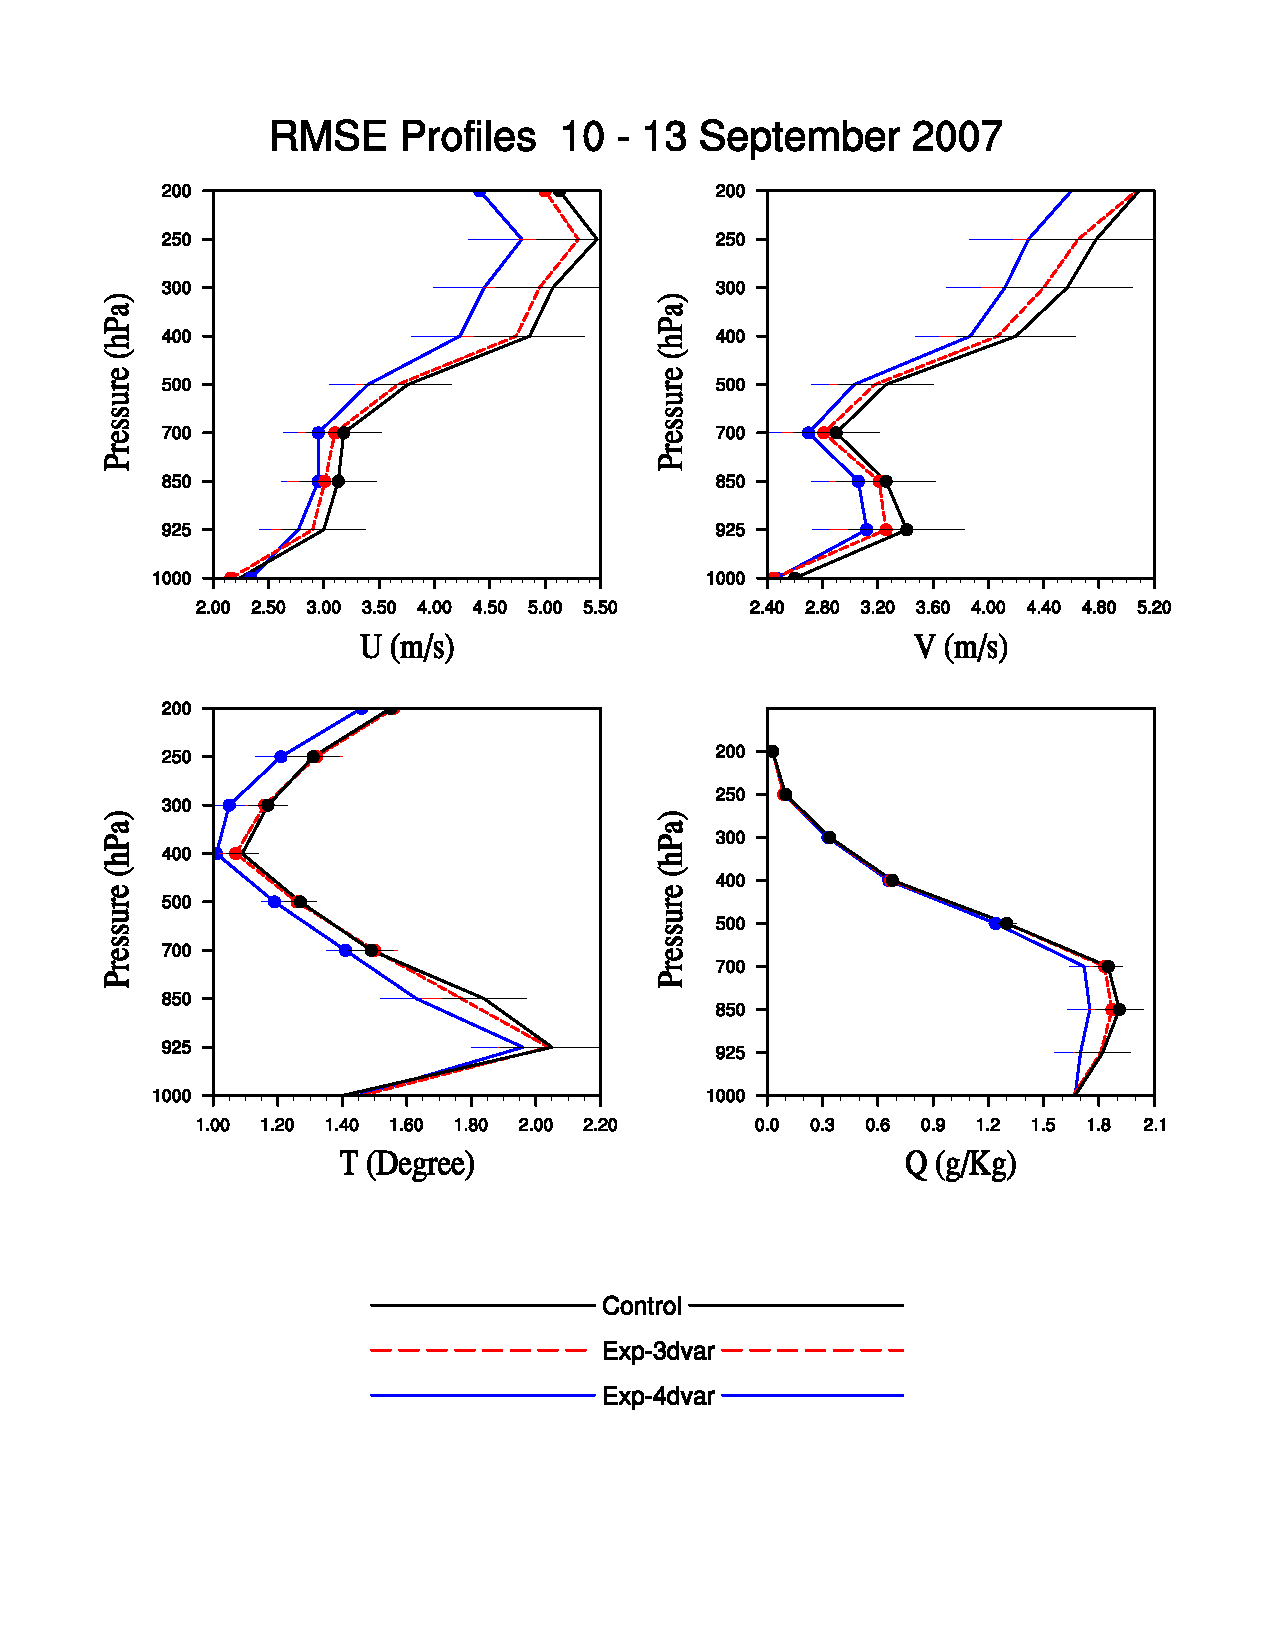
\includegraphics[scale=0.8, trim=0 50 0 80, clip]{Profile_RMSE_30.pdf}
\caption{Profile RMSE at 30h}
\label{30h}
\end{center}
\end{figure}

\begin{figure}
\begin{center}
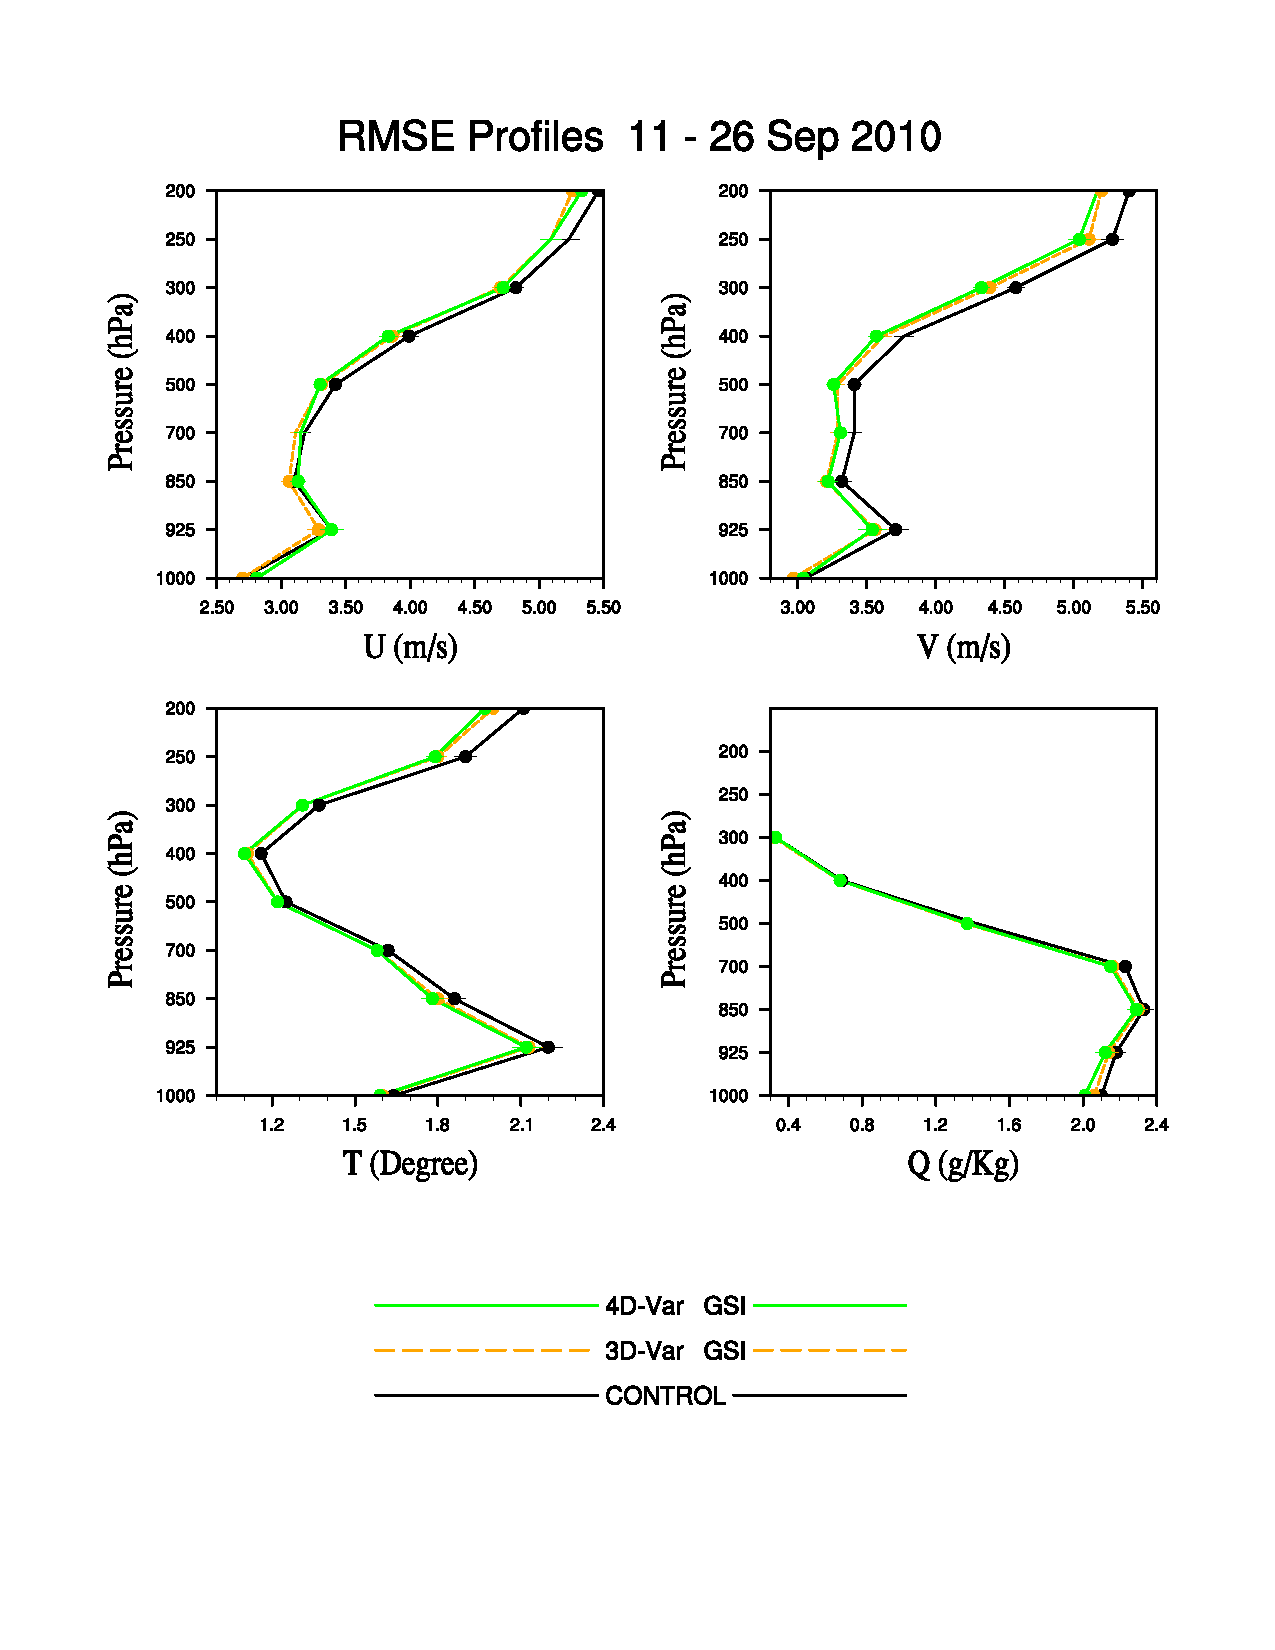
\includegraphics[scale=0.8, trim=0 50 0 80, clip]{Profile_RMSE_36.pdf}
\caption{Profile RMSE at 36h}
\label{36h}
\end{center}
\end{figure}

\begin{figure}
\begin{center}
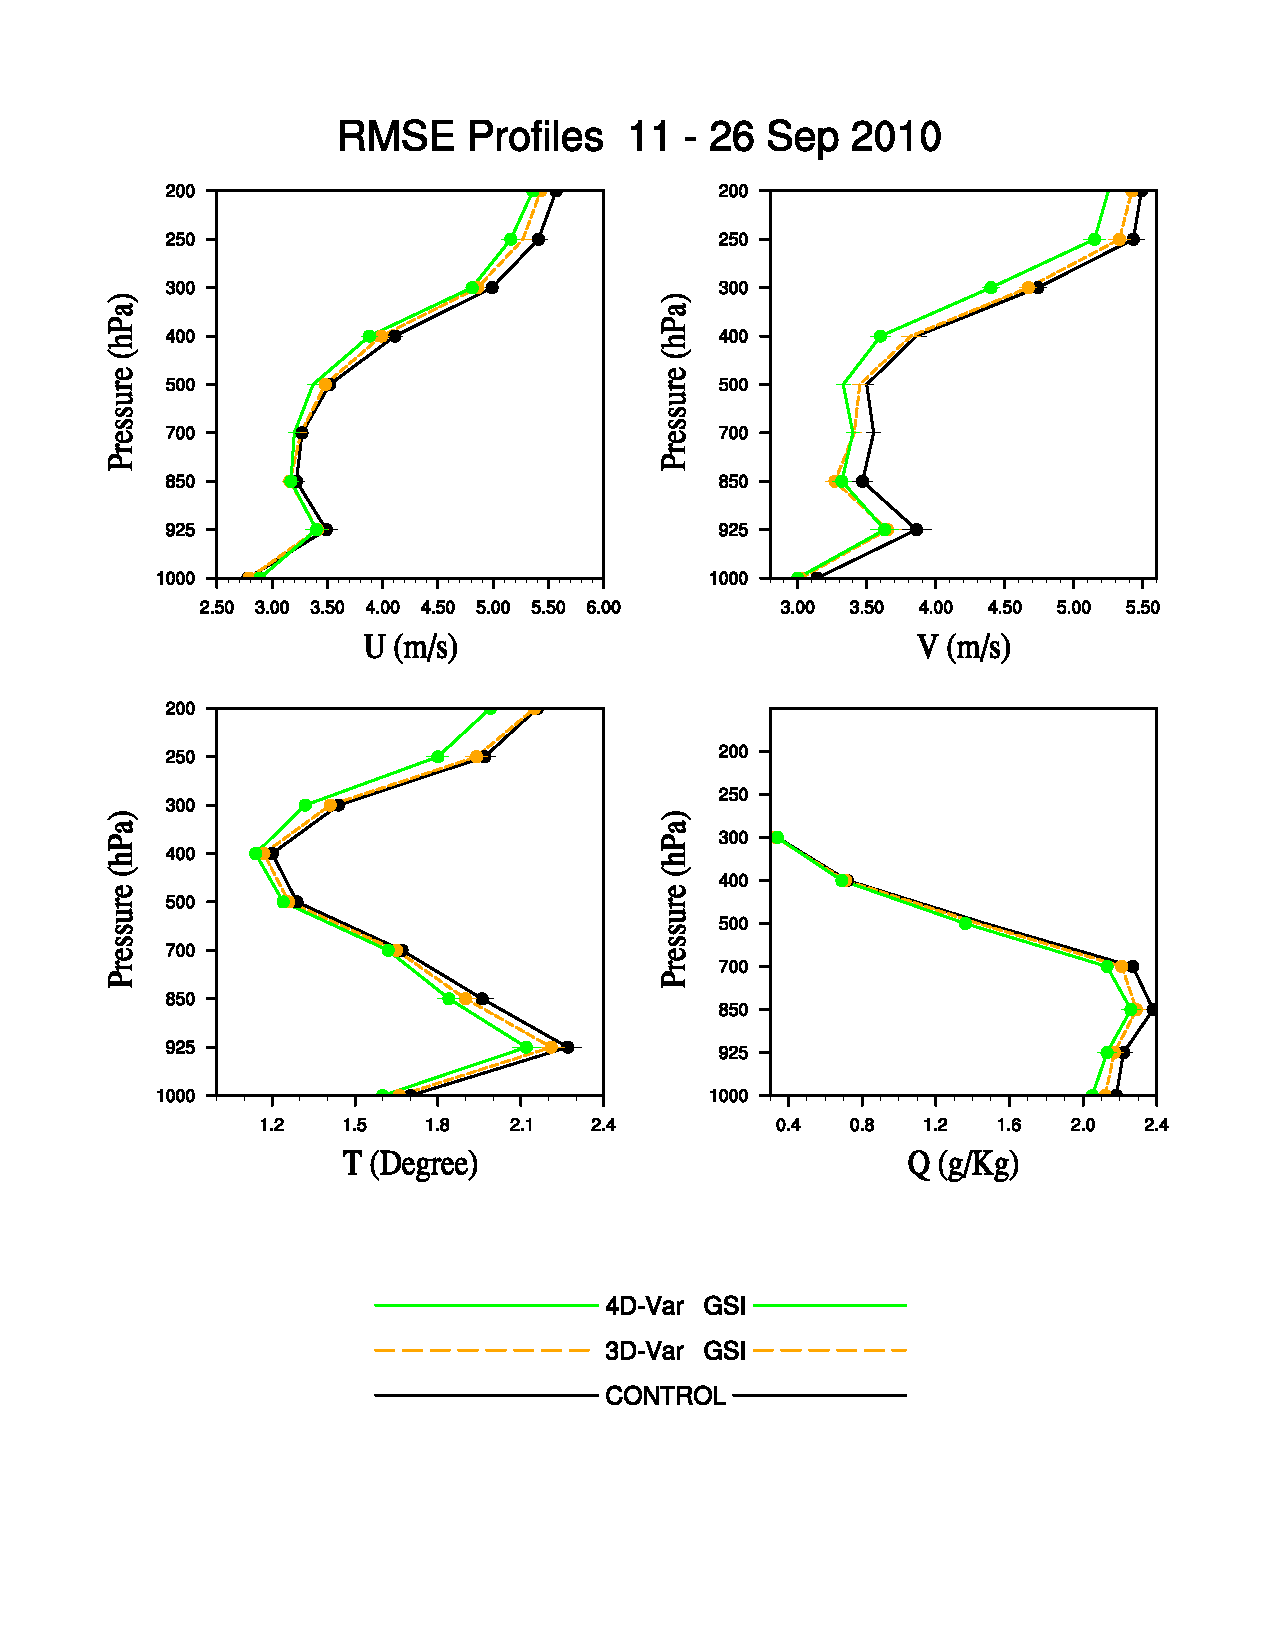
\includegraphics[scale=0.8, trim=0 50 0 80, clip]{Profile_RMSE_42.pdf}
\caption{Profile RMSE at 42h}
\label{42h}
\end{center}
\end{figure}

\begin{figure}
\begin{center}
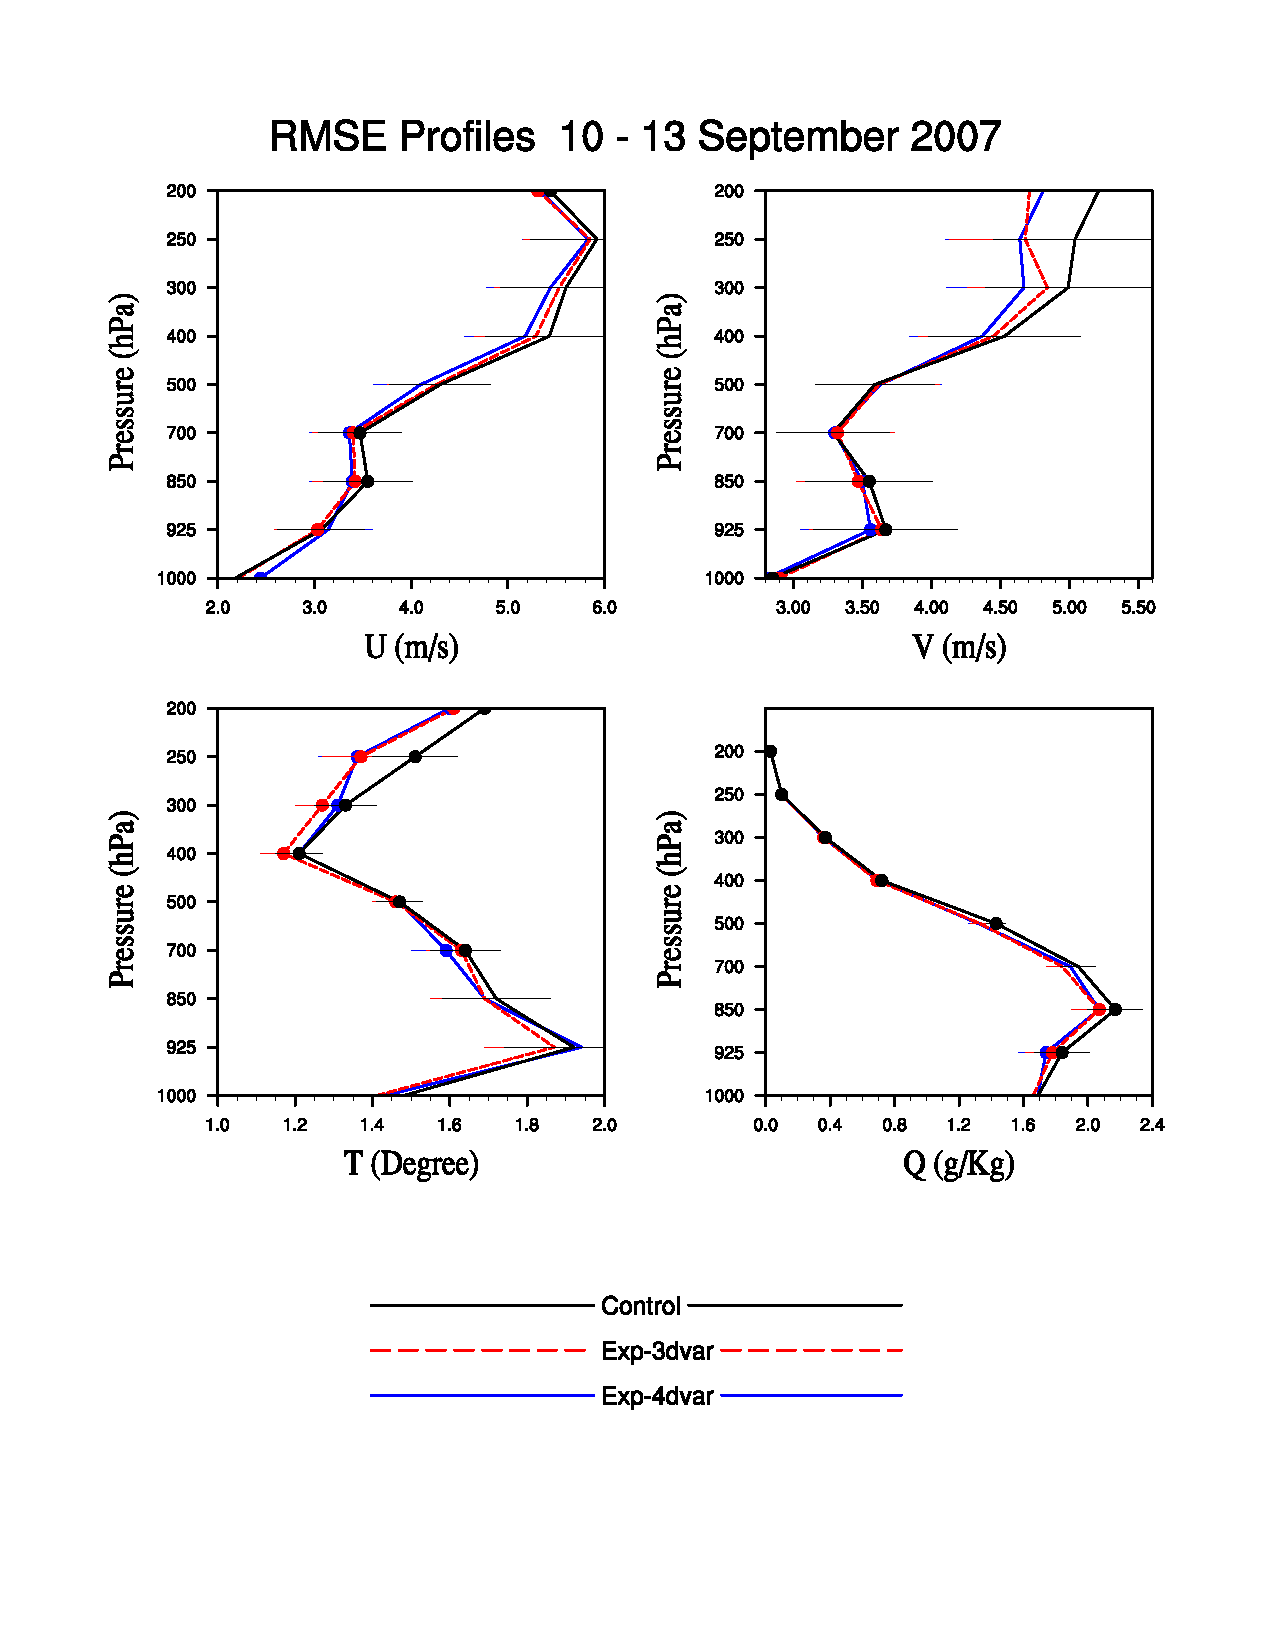
\includegraphics[scale=0.8, trim=0 50 0 80, clip]{Profile_RMSE_48.pdf}
\caption{Profile RMSE at 48h}
\label{48h}
\end{center}
\end{figure}
 
\end{document}